\bb
\begin{samepage}
\ii For each of the following functions $T$, decide whether $T$ is linear. If yes, provide a proof; if no, given an explicit example that violates one of the axioms.  
\bb
\ii $T\colon M_{nn}\rightarrow M_{nn}$, $T(A)=A^2$ 
\ii $T\colon M_{nn}\rightarrow \R$, $T(A)=\tr A$
\ii $T\colon M_{nn}\rightarrow \R$, $T(A)=\det A$. 
\ii $T\colon F((-\infty, \infty))\rightarrow F((-\infty, \infty))$, $T(f)=1+f$
\ii $T\colon F((-\infty, \infty))\rightarrow F((-\infty, \infty))$, $T(f(x))=f(x+3)$
\ee
\end{samepage}
\begin{solution}
\noindent
(a) Nonlinear. Take $A=I_2$. Then $T(2A)=4I\ne 2T(A)=2I$. 
\\
(b) Linear. Easy proof. 
\\
(c) Nonlinear. Let $A=I_2$. Then $\det(2A)=4\ne 2\det(A)=2$. 
\\
(d) Nonlinear. Notice that $T(\boldzero)=1\ne\boldzero$; yet any linear transformation sends the zero vector to the zero vector. 
\\
(e) Linear. 
\begin{align*}
T(cf+dg)&=(cf+g)(x+3)&\text{(by def)}\\
&=cf(x+3)+dg(x+3)&\text{(function arith.)}\\
&=cT(f)+dT(g) &\text{(by def)}
\end{align*}
\end{solution}
\begin{samepage}
\ii Let $(V,\angvec{ \ , })$ be an inner product space. Recall in this context that we define $\norm{\boldv}=\sqrt{\angvec{\boldv, \boldv}}$, and $d(\boldv, \boldw)=\norm{\boldv-\boldw}$. 
\\
An {\bf isometry}  of $V$ is a function $f\colon V\rightarrow V$ that preserves distance: i.e., 
\[
d(f(\boldv), f(\boldw))=d(\boldv, \boldw) \text{ for all <m>\boldv, \boldw\in V</m>}.
\]
In this exercise we will show that any isometry that maps $\boldzero$ to $\boldzero$ is a linear transformation. To that end, assume from now on that $f$ is an isometry of $V$ satisfying $f(\boldzero)=\boldzero$.  
\bb
\ii Prove that $\norm{f(\boldv)}=\norm{\boldv}$: i.e., $f$ preserves norms. 
\ii Prove $\angvec{f(\boldv), f(\boldw)}=\angvec{\boldv, \boldw}$: i.e., $f$ preserves inner products. 
\\
Hint: first prove that $\angvec{\boldv, \boldw}=\frac{1}{2}(\norm{\boldv}^2+\norm{\boldw}^2-\norm{\boldv-\boldw}^2)$.
\ii To prove $f$ is linear it is enough to show $f(\boldv+c\boldw)=f(\boldv)+cf(\boldw)$ for all $\boldv, \boldw\in V$, $c\in \R$. \\
To do so, use the above parts to show that 
\[
\norm{f(\boldv+c\boldw)-(f(\boldv)+cf(\boldw))}=0.
\]  
\noindent
Hint: regroup this difference in a suitable manner so that you can use parts (a)-(b) once you expand out $\norm{\hspace{5pt}}^2$. 
\ee
\end{samepage}
\begin{solution}
Done in class! 
\end{solution}
\begin{samepage}
\ii
\label{Ex:refl} {\em Reflections in $\R^2$}. Given a fixed angle $\alpha$, $0\leq \alpha<\pi $, let $\ell_{\alpha}$ be the line through the origin that makes an angle of $\alpha$ with the positive $x$-axis. 

We define $T_{\alpha}\colon\R^2\rightarrow \R^2$ as 
\[
T_\alpha(\boldx)=\text{ the reflection of <m>\boldx</m> through $\ell_\alpha$}
\]
\bb
\ii Use the previous exercise to show that $T$ is linear. 

\ii Use the recipe to compute the matrix $A_{\alpha}$ such that $T_\alpha=T_{A_\alpha}$.  You will want to draw a picture to see what the action of $T_\alpha$ on $\bolde_1, \bolde_2$ is. 
\ee
\end{samepage}
\begin{solution}
\ \\
It is easiest to see what reflection does by thinking in terms of polar coordinates. Recall: a vector $\boldv$ is completely determined by its length $r=\norm{\boldv}$ and the angle $\theta$ it makes with respect to the positive $x$-axis. (The angle $\theta$ is well-defined only up to multiples of $2\pi$.) The values $r$ and $\theta$ are called polar coordinates of the vector. 
\\
The reflection of $\boldv$ through $\ell_{\alpha}$ is obtained by first rotating it so that it points along $\ell_{\alpha}$, and then rotating again in the same direction by the same amount. As described, it is clear that reflection is an isometry that fixes the origin. It follows from the previous exercise that reflection is thus a linear transformation. 
\\
In more quantitative terms, 
if $\boldv$ makes an angle of $\theta$ with the $x$-axis, then to rotate $\boldv$ to point along $\ell_{\alpha}$ we rotate by an angle of $(\alpha-\theta)$. To get to the reflection we add the same angle $(\alpha-\theta)$ again. In all we have changed the angle $\theta$ to $\theta+2(\alpha-\theta)=2\alpha-\theta$. 
\\
Thus $\bolde_1$, which has $\theta=0$ gets mapped to $T_{\alpha}(\bolde_1)$, a unit vector with angle $2\alpha$; and $\bolde_2$, which $\theta=\pi/2$ gets mapped to $T_{\alpha}(\bolde_2)$, which angle $2\alpha-\pi/2$.
\\ 
Using the recipe 

The matrix we get is 
\[
A_\alpha=\begin{bmatrix}[rr]
\cos(2\alpha)&\cos(2\alpha-\pi/2))\\
\sin(2\alpha)&\sin(2\alpha-\pi/2)
\end{bmatrix}
=
\begin{bmatrix}[rr]
\cos(2\alpha)&\sin(2\alpha)\\
\sin(2\alpha)&-\cos(2\alpha)
\end{bmatrix}
\]
\end{solution}

\ii Let $T\colon \R^3\rightarrow \R^3$ be the transformation defined as $T(\boldv)=\boldw$ where the $\boldw$ is the orthogonal projection of $\boldv$ onto the plane $W\colon x+y+z=0$. 

You can take as a fact that $T$ is a {\em linear transformation}.
\\ 
(a) Find the matrix $A$ such that $T=T_A$. 
\\
(b) Use $A$ to compute the orthogonal projection of $(1,-5,2)$ on the plane $x+y+z=0$. 
\\
(c) Compute $\NS(T)$ and $\range(T)$. 
\\
\begin{solution}
As usual, we have 
\[
A=\begin{bmatrix}
\vert &\vert&\vert \\
T(\bolde_1) &T(\bolde_2)&T(\bolde_3)\\
\vert &\vert &\vert
\end{bmatrix}
\]
where $\bolde_1=(1,0,0)$, $\bolde_2=(0,1,0)$, $\bolde_3=(0,0,1)$. 

Now to compute $T(\bolde_i)$ for each $i$ we use the method from Chapter 3 for projecting a vector onto a plane: namely subtract the projection of $\bolde_i$ onto the normal vector $\boldn=(1,1,1)$ from $\bolde_i$. After some computation we get 
\begin{align*}
T(\bolde_1)&=(2/3,-1/3,-1/3)\\
T(\bolde_2)&=(-1/3,2/3,-1/3)\\
T(\bolde_3)&=(-1/3,-1/3,2/3)
\end{align*}
Thus 
\[ A=\frac{1}{3}\begin{bmatrix}[rrr]
2&-1&-1\\
-1&2&-1\\
-1&-1&2
\end{bmatrix}
.
\]
Nifty! This means to compute the orthogonal projection of $(x,y,z)$ onto the plane $x+y+z=0$ we just compute $A\begin{bmatrix}
x\\ y\\ z
\end{bmatrix}$.

Thus, for example, \[
T(1,-5,2)=A\begin{bmatrix}[r]
1\\ -5 \\ 2
\end{bmatrix}=\begin{bmatrix}[r]
5/3\\ -13/3 \\ 8/3
\end{bmatrix}.
\]
%Here is a picture to convince you! Plane and its normal vector in green.
%\[
%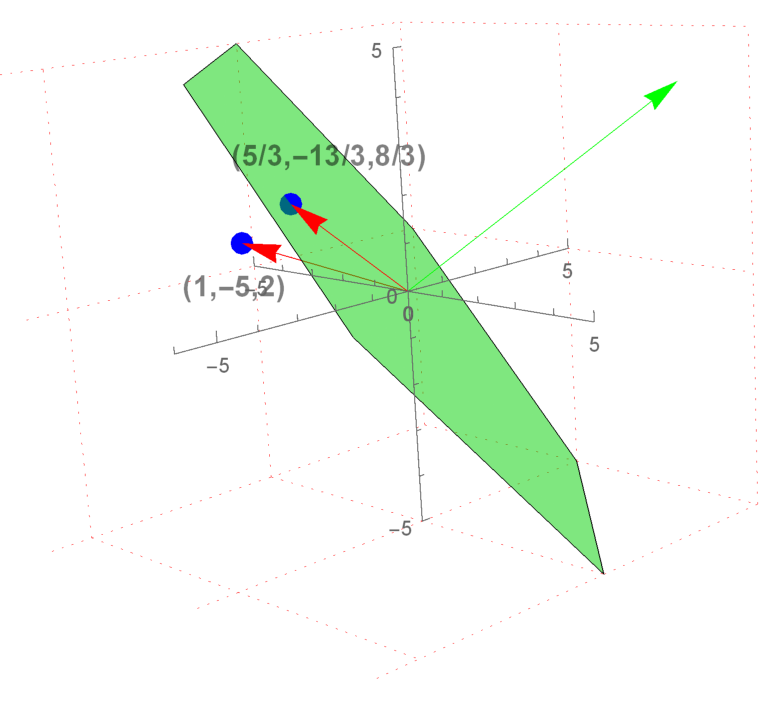
\includegraphics[width=3in]{OrthoProj}
%\]
To determine $\NS(T)$ and $\range(T)$ we can proceed either (1) conceptually, or (2) algebraically. 

Conceptually, we have shown previously that for any orthogonal projection $\text{proj}_W$ we have 
\begin{align*}
\proj{\boldv}{W}=\boldzero&\Longleftrightarrow \boldv\in W^\perp, \text{ and }\\
\proj{\boldw}{W}=\boldw&\text{for all } \boldw\in W
\end{align*}
From these two facts it follows easily that $\NS(T)=W^\perp=\Span(\{(1,1,1)\})$ and $\range(T)=W$.

Algebraically, since $T=T_A$ where $A$ is the matrix above, it follows that 
\begin{align*}
\NS(T)&=\NS(A)\\
\range(T)&=\CS(A)
\end{align*}
and we can compute these using the usual fundamental space algorithms. We get $\NS(A)=\Span(\{(1,1,1)\}$ and $\CS(A)=\Span(\{(2/3,-1/3,-1/3),(-1/3,2/3,-1/3)\})$. These are of course the line through $(1,1,1)$ and the plane $x+y+z=0$, respectively. 
 
\end{solution}

\ii Let $T\colon V\rightarrow W$ be a linear transformation. 
\bb
\ii Prove that $\NS(T)$ is a subspace of $V$. 
\ii Prove that $\range(T)$ is a subspace of $W$. 
\ee
%\vfill
\begin{solution}
\noindent We proved (b) in lecture. Part (a) is easy. 
\end{solution}
\ii Use the rank-nullity theorem to compute the rank of the linear transformation $T$ described. 
\bb
\ii $T\colon\R^7\rightarrow M_{32}$ has nullity 2.
\ii $T\colon P_3\rightarrow \R$ has nullity 1.
\ii The null space of $T\colon P_5 \rightarrow P_5$ is $P_4$.
\ii $T\colon P_n\rightarrow M_{mn}$ has nullity 3.
\ee
\begin{solution}
\noindent
(a)
$\rank(T) = \dim(R^7) - 2 = 7-2=5$
\\
(b)
$\rank(T) = \dim(P_3) - 1 = 4-1=3$
\\
(c)$\rank(T) = \dim(P_5) - \nullity(T) = \dim(P_5)-\dim(P_4) = 1$
\\
(d) 
$\rank(T) = \dim(P_n)-3 = (n+1) - 3 = n-2$
\end{solution}

\ii Let $T\colon V\rightarrow W$ be a linear transformation, where $V$ is finite dimensional.\\
Let $S=\{\boldv_1,\boldv_2,\dots, \boldv_r\}$ be a basis of $\NS(T)$ and this basis to a full basis $B=\{\boldv_1,\boldv_2,\dots, \boldv_r, \boldu_{1},\dots \boldu_{n-r}\}$ of $V$. 
\\
Prove the claim made in my lecture notes: namely, that  $S'=\{T(\boldu_{1}),\dots, T(\boldu_{n-r})\}$ is a basis of $\range(T)$.
\\
Treat the linear independence and span questions separately. \\
For the spanning question, begin as follows: given $\boldw\in \range(T)$, by definition there is a $\boldv\in V$ such that $T(\boldv)=\boldw$; write out $\boldv$ in terms of the basis $B$ and go from there. 
%\vfill
\begin{solution}
\noindent We prove separately that (a) $S'$ is linearly independent, and (b) $S'$ spans $\range(T)$. 
\\
(a) Suppose we have $\sum_{i=1}^{n-r}c_iT(\boldu_i)=\boldzero$. Then $T(\sum_{i=1}^{n-r}c_i\boldu_i)=\boldzero$, and we see that the vector $\boldu=\sum_{i=1}^{n-r}c_i\boldu_i\in\NS(T)$. Since the $\boldv_i$ span $\NS(T)$ we then also have 
\[
\boldu=\sum_{i=1}^rd_i\boldv_i \text{ for some <m>d_i\in\R</m>}.
\]
It would stand to reason, since $S$ is a basis, that the only way can have 
\[
\boldu=\sum_{i=1}^rd_i\boldv_i=\sum_{i=1}^{n-r}c_i\boldu_i
\]
is if $d_i=c_j=0$ for all $i, j$. But how can we prove this? The equality above implies 
\[
d_1\boldv_1+d_2\boldv_2+\cdots +d_r\boldv_r-c_1\boldu_1-c_2\boldu_2-\cdots -c_{n-r}\boldu_{n-r}=\boldzero.
\]
By linear independence of $S$ it now follows that $d_i=c_j=0$ for all $i, j$. 
\\
(b) First, since $S'\subseteq \range(T)$, we have $\Span(S')\subseteq \range(T)$. To show the other direction, take any $\boldw\in \range(T)$. Then $\boldw=T(\boldv)$ for some $\boldv\in V$. Since $S$ is a basis for $V$, we can write 
\[
\boldv=c_1\boldv_1+c_2\boldv_2+\cdots c_r\boldv_r+d_1\boldu_1+d_2\boldu_2+\cdots +d_{n-r}\boldu_{n-r}
\]
for some $c_i, d_j\in\R$. Then we have 
\begin{align*}
\boldw&=T(\boldv)\\
&=T(c_1\boldv_1+c_2\boldv_2+\cdots c_r\boldv_r+d_1\boldu_1+d_2\boldu_2+\cdots +d_{n-r}\boldu_{n-r})\\
&=c_1T(\boldv_1)+c_2T(\boldv_2)+\cdots c_rT(\boldv_r)+d_1T(\boldu_1)+d_2T(\boldu_2)+\cdots +d_{n-r}T(\boldu_{n-r})\\
&=\boldzero+d_1T(\boldu_1)+d_2T(\boldu_2)+\cdots +d_{n-r}T(\boldu_{n-r})  &\text{(since <m>T(\boldv_i)=\boldzero</m> for all $i$)}\\
&=d_1T(\boldu_1)+d_2T(\boldu_2)+\cdots +d_{n-r}T(\boldu_{n-r})
\end{align*}
This shows $\boldw\in \Span(S')$, as desired. 
\end{solution} 
\begin{samepage}
\ii Let $V=\R^\infty=\{(a_1,a_2,\dots, )\colon a_i\in\R\}$, the space of all infinite sequences. Define the ``shift left" and ``shift right" functions as follows:
\begin{align*}
T_L\colon \R^\infty&\rightarrow \R^\infty\\
s=(a_1,a_2, a_3,\dots )&\longmapsto T_L(s)=(a_2, a_3,\dots) \\
\\
T_R\colon \R^\infty&\rightarrow \R^\infty\\
s=(a_1,a_2, a_3,\dots )&\longmapsto T_R(s)=(0,a_1,a_2,\dots) 
\end{align*}
\bb
\ii Prove that $T_L$ and $T_R$ are linear. 
\ii Show that $T_L$ is onto, but not one-to-one. (Compute $\NS(T_L)$ and $\range(T_L)$.)
\ii Show that $T_R$ is one-to-one, but not onto. (Compute $\NS(T_R)$ and $\range(T_R)$. )
\ii Show that $T_L\circ T_R=I_{\R^\infty}$ but $T_R\circ T_L\ne I_{\R^\infty}$. 
\ee
\end{samepage}
\begin{solution}
\noindent {\em Moral of this exercise}: when $V$ is NOT finite-dimensional, we do NOT necessarily have the equivalence
\[
\text{<m>T</m> invertible iff $T$ onto iff $T$ 1-1}.
\]
for linear transformations $T\colon V\rightarrow V$.  
\\
(a) Easy. 
\\
(b) Given any sequence $t=(b_1,b_2,\dots )$, we have $b=T(s)$, where $s=(0,b_1,b_2,\dots)$. Thus $T_L$ is onto: i.e., $\range(T_L)=\R^\infty$. It is east to see that $T_L$ is not 1-1: in fact, we compute easily $\NS(T_L)$ is the subspace of infinite sequences of the form $(c,0,0,\dots)$, which is nontrivial. 
\\
(c) We have $T_R((a_1,a_2,\dots))=(0,0,\dots)$ iff $(0,a_1,a_2,\dots)=(0,0,\dots)$ if and only if $a_1=a_2=\cdots =0$. This shows $\NS(T_R)=\{\boldzero\}$. It is also clear that $\range(T_R)$ is the space of all infinite sequences of the form $(0,b_1,b_2,\dots)$. As this is not all of $\R^\infty$, we see that $T_R$ is not onto. 
\\
(d) Also easy. This is an example of a function ($T_R)$ that has a left-inverse (namely, $T_L$) which is not a right-inverse (since $T_R\circ T_L\ne I_V$)!! Funny things can happen when $V$ is not finite-dimensional. 
\end{solution}
\ii (Coordinate vectors) Let $V$ be finite-dimensional. Choose any basis $B=\{\boldv_1,\boldv_2,\dots , \boldv_n\}$.
\\
Show that taking coordinate vectors defines an isomorphism from $V$ to $\R^n$. 
\\
That is, define $T\colon V\rightarrow \R^n$ by $T(\boldv)=[\boldv]_B$, and show $T$ is an isomorphism. (Note: you must first show $T$ is a linear transformation!) 
\\
\begin{solution}
\noindent We showed $T=[\hspace{8pt}]_B$ was linear in an earlier homework exercise. 
\\
Since $\dim(V)=\dim(\R^n)=n$, to show $T$ is invertible (or an isomorphism), it suffices to show either that it is onto, or that it is 1-1. I'll prove the former. Given any vector $(a_1,a_2,\dots, a_n)\in\R^n$ we need to show there is a vector $\boldv$ such that $[\boldv]_B=(a_1,a_2,\dots, a_n)$. That's easy: take $\boldv=a_1\boldv_1+\cdots +a_n\boldv_n$. 

\end{solution}

\ii (Transpose) Define $S\colon M_{mn}\rightarrow M_{nm}$ by $S(A)=A^T$. Show that $S$ is an isomorphism. 
%\vfill
\begin{solution}
\ \\
Define the linear transformation $\hat{S}\colon M_{nm}\Rightarrow M_{mn}$ as $\hat{S}(B)=B^T$. Then 
\begin{align*}
\hat{S}(S(A))&=\hat{S}(A^T)=(A^T)^T=A, \text{ and }\\
S(\hat{S}(B))&=S(B^T)=(B^T)^T=B,
\end{align*} 
showing $\hat{S}$ is the inverse of $S$, and hence that $S$ is invertible. 
\end{solution}
\ii (Conjugation). Fix an invertible matrix $Q\in M_{nn}$. Define $T\colon M_{nn}\rightarrow M_{nn}$ as $T(A)=QAQ^{-1}$. Show $T$ is an isomorphism. (This operation is called {\bf conjugation by $Q$}.) 
\\
\begin{solution}
\ \\
\end{solution}
\ii (Evaluation). Let $V=P_n$. Let $c_1,c_2,\dots, c_{n+1}$ be any distinct constants. Show that the map 
\begin{align*}
T\colon P_n&\rightarrow \R^{n+1}\\
p(x)&\mapsto (p(c_1), p(c_2), \dots, p(c_{n+1})
\end{align*}
is an isomorphism. 

(Note: this isomorphism tells us that a degree $n$ polynomial $p(x)$ is uniquely determined by its values at any choice of $n+1$ distinct inputs. )
%\vfill
\\
\begin{solution}
%\ \\
\noindent Note: it is easy to show that $T$ is actually a linear transformation. 
\\
To show $T$ is invertible (or an isomorphism), it is enough to show that $\NS(T)$ is trivial (since $\dim P_n=\dim\R^{n+1}=n+1$). 
\\
Suppose $T(p)=\boldzero$. Then $p(c_1)=p(c_2)=\cdots =p(c_{n+1})=0$. But then the polynomial $p(x)$ has $n+1$ distinct roots. But a nonzero polynomial of degree $r\leq n$ can have at most $n$ distinct roots. It follows that $p(x)$ must be the zero polynomial, and hence that $\NS(T)$ is trivial. 
\end{solution}
\ii Fix any $c\in\R$ and define $T\colon F((-\infty, \infty))\rightarrow F((-\infty, \infty))$ as $T(f)=g$, where $g(x)=f(x+c)$. (Thus $T$ is the ``shift by $c$" operator on function space.)  
\bb
\ii Show that $T$ is linear. 
\ii Prove $T$ is invertible by providing its inverse. 
\ee
\begin{solution}
%\ \\
\noindent 
(a) Easy. 
\\
(b) The inverse is defined as $S(g)=h(x)$, where $h(x)=g(x-c)$. 
\end{solution}
\ii Show that a matrix transformation $T_A\colon\R^n\rightarrow \R^n$ is invertible (as a linear transformation) if and only if $A$ is invertible (as a matrix). 
\\
Thus invertibility in the matrix sense is the same thing as invertibility in the linear transformation sense. 
%\vfill
\\
\begin{solution}
%\ \\
\noindent
Observe that $\NS(T_A)=\NS(A)$. Then by our various invertibility theorems
\begin{align*}
T_A \text{ invertible}&\Leftrightarrow \NS(T_A)=\{\boldzero\} &\text{(invertibility theorem for linear trans.)}\\
&\Leftrightarrow \NS(A)=\{\boldzero\} \\
&\Leftrightarrow A \text{ invertible} &\text{(IV Theorem for matrices)}
\end{align*}
Note: we can further say that the inverse of $T_A$ in this case is $T_{A^{-1}}$.
\end{solution}
\ii Show that if $T\colon V\rightarrow W$ is an isomorphism, and $B=\{\boldv_1,\boldv_2,\dots,\boldv_n\}\subseteq V$ is a basis for $V$, then $T(B)\subseteq W$ is a basis for $W$. 
\\
\begin{solution}
\noindent The notation $T(B)$ denotes the set $B'=\{T(\boldv_1),T(\boldv_2),\dots,T(\boldv_n)\}$. To show $B'$ is a basis, we must show the vectors $\boldw_i=T(\boldv_i)$ both span $W$ and are linearly independent. 
\\	
We can make one shortcut. Since $\#B=n$ we have $\dim(V)=n$. Since $T$ is an {\em isomorphism} and $\dim(V)=n$, we must also have $\dim(W)=n$. Lastly, since $\# B'=n=\dim(W)$ we need only show either that $B'$ spans {\em or} that it is linearly independent. 
\\	
I will show that $T(B)$ spans $W$. To this end take any $\boldw\in W$. We must show that we can write $\boldw$ as a linear combination of the $\boldw_i$. 
\\	
Since $T$ is invertible, it is onto. Thus there is a $\boldv\in V$ such that $T(\boldv)=\boldw$. Since $B$ is a basis of $V$, we can write $\boldv=a_1\boldv_1+a_2\boldv_2+\cdots +a_n\boldv_n$. But then we have 
	\begin{align*}
	\boldw&=T(\boldv)\\
	&=T(a_1\boldv_1+a_2\boldb_2+\cdots +a_n\boldv_n)\\
	&=a_1T(\boldv_1)+a_2T(\boldb_2)+\cdots +a_nT(\boldv_n) &\text{(since <m>T</m> is linear)}\\
	&=a_1\boldw_1+a_2\boldw_2+\cdots +a_n\boldw_n &\text{(by def. <m>\boldw_i=T(\boldv_i)</m>},
	\end{align*} 
	and this shows $w$ is a linear combination of the $\boldw_i$, as desired. 
	
\end{solution}

\ee